% ***********************************************************
% ******************* PHYSICS HEADER ************************
% ***********************************************************
% Version 2
\documentclass[9pt,twocolumn]{article} 
\usepackage{amsmath} % AMS Math Package
\usepackage{amsthm} % Theorem Formatting
\usepackage{amssymb}	% Math symbols such as \mathbb
\usepackage{graphicx} % Allows for eps images
\usepackage{multicol} % Allows for multiple columns
\usepackage{lipsum}
\usepackage{adjustbox}
\usepackage{abstract}
\usepackage{multicol}
\usepackage[table,xcdraw]{xcolor}
\usepackage{subcaption}
\usepackage[dvips,letterpaper,margin=0.75in,bottom=0.5in]{geometry}
 % Sets margins and page size
\pagestyle{empty} % Removes page numbers
\makeatletter % Need for anything that contains an @ command 
\renewcommand{\maketitle} % Redefine maketitle to conserve space
{ \begingroup \vskip 10pt \begin{center} \large {\bf \@title}
	\vskip 10pt \large \@author \hskip 20pt \@date \end{center}
  \vskip 10pt \endgroup \setcounter{footnote}{0} }
\makeatother % End of region containing @ commands
\renewcommand{\labelenumi}{(\alph{enumi})} % Use letters for enumerate
% \DeclareMathOperator{\Sample}{Sample}
\let\vaccent=\v % rename builtin command \v{} to \vaccent{}
\renewcommand{\v}[1]{\ensuremath{\mathbf{#1}}} % for vectors
\newcommand{\gv}[1]{\ensuremath{\mbox{\boldmath$ #1 $}}} 
% for vectors of Greek letters
\newcommand{\fd}[1]{\mathbf{#1}}
\newcommand{\uv}[1]{\ensuremath{\mathbf{\hat{#1}}}} % for unit vector
\newcommand{\abs}[1]{\left| #1 \right|} % for absolute value
\newcommand{\avg}[1]{\left< #1 \right>} % for average
\let\underdot=\d % rename builtin command \d{} to \underdot{}
\renewcommand{\d}[2]{\frac{d #1}{d #2}} % for derivatives
\newcommand{\dd}[2]{\frac{d^2 #1}{d #2^2}} % for double derivatives
\newcommand{\pd}[2]{\frac{\partial #1}{\partial #2}} 
% for partial derivatives
\newcommand{\pdd}[2]{\frac{\partial^2 #1}{\partial #2^2}} 
% for double partial derivatives
\newcommand{\pdc}[3]{\left( \frac{\partial #1}{\partial #2}
 \right)_{#3}} % for thermodynamic partial derivatives
\newcommand{\ket}[1]{\left| #1 \right>} % for Dirac bras
\newcommand{\bra}[1]{\left< #1 \right|} % for Dirac kets
\newcommand{\braket}[2]{\left< #1 \vphantom{#2} \right|
 \left. #2 \vphantom{#1} \right>} % for Dirac brackets
\newcommand{\matrixel}[3]{\left< #1 \vphantom{#2#3} \right|
 #2 \left| #3 \vphantom{#1#2} \right>} % for Dirac matrix elements
\newcommand{\grad}[1]{\gv{\nabla} #1} % for gradient
\let\divsymb=\div % rename builtin command \div to \divsymb
\renewcommand{\div}[1]{\gv{\nabla} \cdot #1} % for divergence
\newcommand{\curl}[1]{\gv{\nabla} \times #1} % for curl
\let\baraccent=\= % rename builtin command \= to \baraccent
\renewcommand{\=}[1]{\stackrel{#1}{=}} % for putting numbers above =
\newtheorem{prop}{Proposition}
\newtheorem{thm}{Theorem}[section]
\newtheorem{lem}[thm]{Lemma}
\theoremstyle{definition}
\newtheorem{dfn}{Definition}
\theoremstyle{remark}
\newtheorem*{rmk}{Remark}

\begin{document}

%\begin{multicols}{2}
\section{Introduction}
Blob are annoying account for much transport
Why are PIC codes nice?
\section{Stating the physical problem and expectations}
Basic idea
Purpose is to test blob dynamics and verify fluid scaling based on interchange motion. Furthermore, as the FLR effects are an inherent part of the gyromotion they are expected to occur naturally.

In this paper blobs are modelled as Gaussian perturbation in the density and some in the temperature on a uniform background:
\begin{equation}
n(t=0) = n_0+ n_b\exp\left(-\frac{(\fd x-\fd x_c)^2}{2\sigma^2}\right)
\end{equation}
The blob is placed in a static inhomogeneous magnetic field given by:
\begin{equation}
\fd B = -\frac{B_0R_0}{R_0+x}{\fd {\hat{z}}}
\end{equation}
Here $B_0$ is the magnetic field at $R_0$ which is the distance of the blob from the center???????!!!!!!
The gradient arising from this field leads to a grad-B drift of the ions and electrons causing a polarization of the blob in turn creating an electric field 
The problem has been analysed thoroughly using fluid theory and a velocity scaling for the radial propagation of the blob can be found from dimensional analysis of:
\begin{equation}
V_{\perp} \propto \gamma\sigma = c_s\sqrt{\frac{\sigma\Delta n}{R n_0}}
\end{equation}
Where $\gamma=\sqrt{\frac{c_s\Delta n}{\sigma R n}}$ is the interchange rate and $c_s=\sqrt{P/\rho_m}$ is the ion sound speed with $P$ the plasma pressure and $\rho_m$ the plasma mass density.

A typical assumption in the fluid picture is that the plasma is quasineutral, i.e. $|n_i-n_e|\ll 1$. For the code in question this is explicitly met for the system in its entirety but not necessarily on the appropriate length scales. Therefore the definition of quasi neutrality from [cite] is used as a measure:
\begin{equation}
\frac{\Delta n}{n}\leqslant \frac{\lambda_d^2}{L^2}\ll 1
\end{equation}
Where $\lambda_d$ is the Debye length and $L$ is some characteristic length scale which in this case is the Larmor radius. This effectively means that the Debye screening is large within a region of $L^2$. 

FLR effects [MAKE SURE LARMOR RADIUS IS DEFINED BEFORE HAND]:
Due to the mass dependency on the Larmor orbits, ions will have a larger radius than the electron at the same temperature. In the case of the blob perturbation this means that an ion will transverse a larger part of the blob than the electron. As the electric field varies on a scale comparable to the blob width, the field felt by the ions change significantly compared to the field felt by an electron over the course of an orbit. As such the electron experiences an almost homogeneous electric field. The effects arising from this is what is known as finite Larmor radius (FLR) effects. In [madsen, held] an attempt has been made at quantifying effect and numerical results show a secondary drift of the blob in the ion grad-B direction. In this paper we will not do so, but simple give a measure of the FLR effects on the poloidal propagation for comparing different scenarios:
\begin{equation}
\Phi = \frac{x}{y}\sim \frac{v_x}{v_y}
\end{equation}  

\section{Numerics and simulation system}
In this paper the goal is to investigate blob dynamics using a first principle, fully kinetec approach. This means that individual particle motion for both ions and electrons is resolved and so that all physics are inherently resolved in particular the gyromotion and the effects arising from this. This type of simulation is particularly useful when it comes to transport and turbulence simulations as all dynamics are present.
This is in contrast to fluid models where a number of moments are taken of the boltzmann equation, and certain approximations are included to give a coherent picture.

To model this first principles approach an electrostatic Particle-In-Cell code modified from the Photon-Plasma code is used []. This modified version solves the Vlasov equation:
\begin{equation}
\pd ft+\fd v\cdot\gv{\nabla_x}f+\frac{q}{m}\left(\fd E+\fd v\times\fd B\right)\cdot \gv{\nabla_v}f=0
\end{equation}
Where $f(\fd x, \fd v,t)$ is the distribution function for a single particle. The charge of the particles are interpolated onto a spatial grid using cubic spline interpolation. This gives rise to a charge density on the grid which in turn can be used to find the electrical fields. 
Note that the system is assumed collision-less expect for interactions through the particle-grid interpolation. The magnetic field is assumed to be constant and the electric potential is solved for using the Poisson equation:
\begin{equation}
\rho =-\frac{\Delta\phi}{\varepsilon_0}
\end{equation}
Where $\rho$ is the charge density and $\phi$ the electric potential. 
From this the electrical field is found as:
\begin{equation}
\fd E = -\grad \phi
\end{equation}
The grid is staggered in such a way that the electric field is shifted wrt. the density field. And the potential solver is of 6th order.


In the simulations the background density is set to be $n_0=10^{17}m^{-3}$ with a background magnetic field $B_0=1T$. Note that the density is some orders of magnitude smaller than typical densities found in fluid simulations and real worlds problems [cite?]. The reason for this is the computational constraints imposed by stability criteria of PIC codes where both the plasma frequency and the Debye length have to be resolved.


Boundary condition.
The boundary condition for the y-direction are periodic while for the x-direction a Neumann boundary for the electric potential is used and the particles are reflected according to [cite the one with boundary]. The magnetic field on the boundary is as prescribed above. Since the code is a 6th order code in the fields, a number of ghost points are needed outside the domain. The magnetic field is known beforehand due to it being constant.  The charge density is handled as mirror charges, making it possible to find the potential which is also mirrored. From this the electric field, the x-component is found with the ghost points being antisymmetric around zero wrt. the inside field. The y-component is simply reflected [IS THIS TOO DETAILED? PROBABLY].

In the code, the grid is resolved s.t. $\Delta x\approx \lambda_d\approx 5\rho_s$ where $\rho_s=\sqrt{T_e/m_i}/\omega_{ci}$ is the Larmor radius and $\lambda_d$ is the Debye length.

A number of different simulation are carried out to test the different scaling parameters. A common setup is such that the perturbation amplitude is $n_b=n_0$ with a temperature of $T_i=T_e=20 eV$, radius of $R_0=500\rho_s$ and blob width of $\sigma = 5 \rho_s$. To test the various scaling parameters, one parameters is varied while the others are fixed with the above quantities. The used values are; for radius of $R_0/\rho_s = {250,500,1000,2000}$; for perturbation $n_b/n_0 = {0.5,1,2,4}$; for width $\sigma/\rho_s = {2.5,5,10,20}$.

The default grid is such that $x_{min}=-20\rho_S$, $x_{max}=80\rho_S$ and $-y_{min}=y_{max}=37.5\rho_s$, with a total of $512\times 384$ grid points. With this the blob is positioned at $\fd x_c = {0,0}$ so that the magnetic field at the center of the blob is $B_0$. Furthermore, to alleviate computational requirements the mass ratio between the ions and electrons is $m_i/m_e=100$. The charge of the particles are $q_i=q_e$
\section{Numerical Results}
Checking the driving mechanism - potential and electric field - the blob moves - how does it scale - what about FLR effects.

To test scaling the scaling of the radial motion the blob seen in equation [insert eq.] several runs with varying perturbation amplitude, blob width, major radius and ion temperature. The ion temperature dependence is through the sound speed $c_s\propto \sqrt{1+\tau}$ where $\tau = Ti/T_e$.

Snapshots of the density evolution of blob simulation with the default values stated above is seen in fig... As seen the seeded blob moves radially outwards and starts forming a plume like structure. This is similar to results seen in e.g. [jens, held etc.] and corresponds with what is expected for density inhomogeneities in an inhomogeneous magnetic field such as this. 

\begin{figure*}[h]
  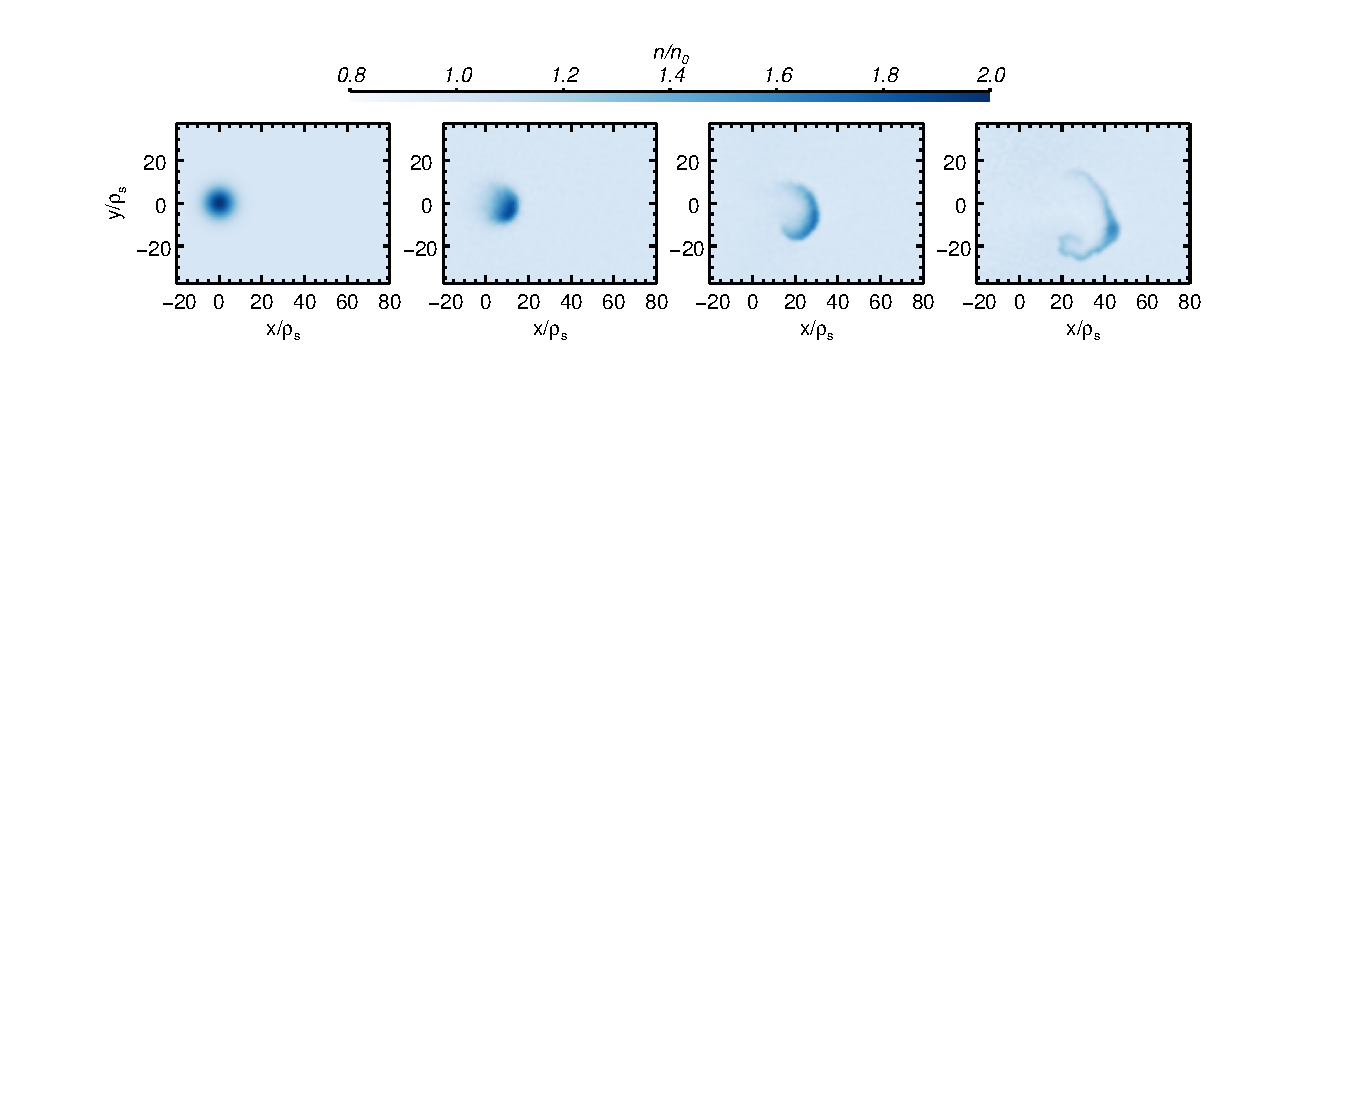
\includegraphics[trim=0mm 128mm 0mm 0mm,width=\textwidth]{Pictures/fourcontour.eps}
  \caption{Ion density profiles at $t\omega_{ci}={0,150,300,450}$}
  \label{blob}
\end{figure*}

\begin{figure*}[h]
  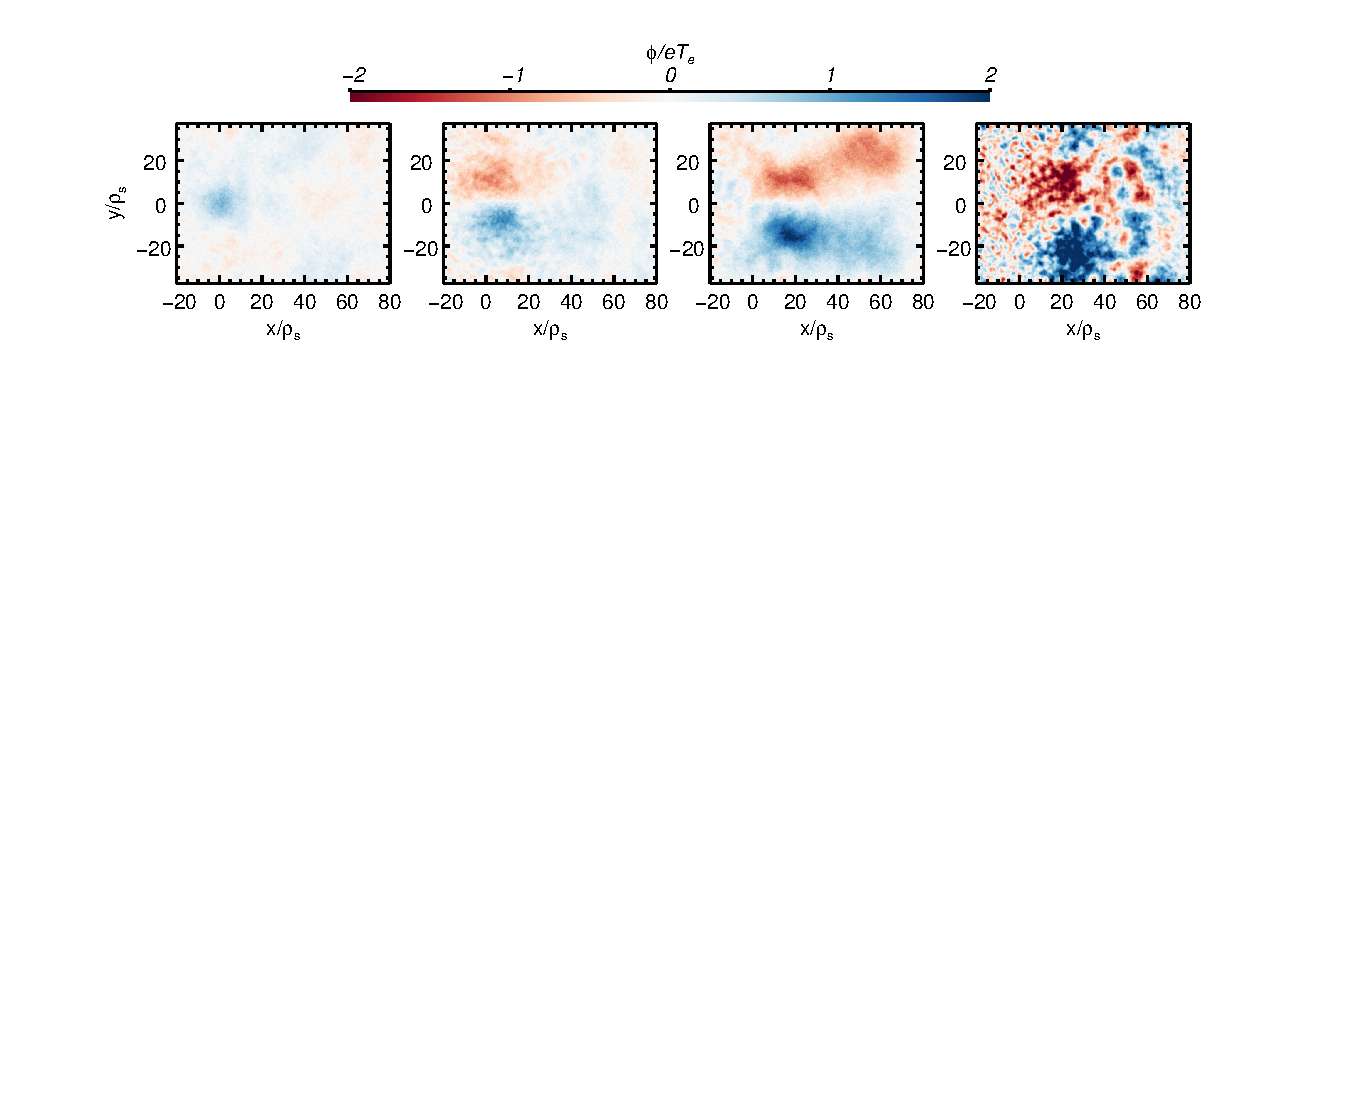
\includegraphics[trim=0mm 128mm 0mm 0mm,width=\textwidth]{Pictures/threephitot.eps}
  \caption{Gyroaveraged potential at $t\omega_{ci}={6,150,300,450}$}
  \label{pot}
\end{figure*}

\begin{figure*}[h]
  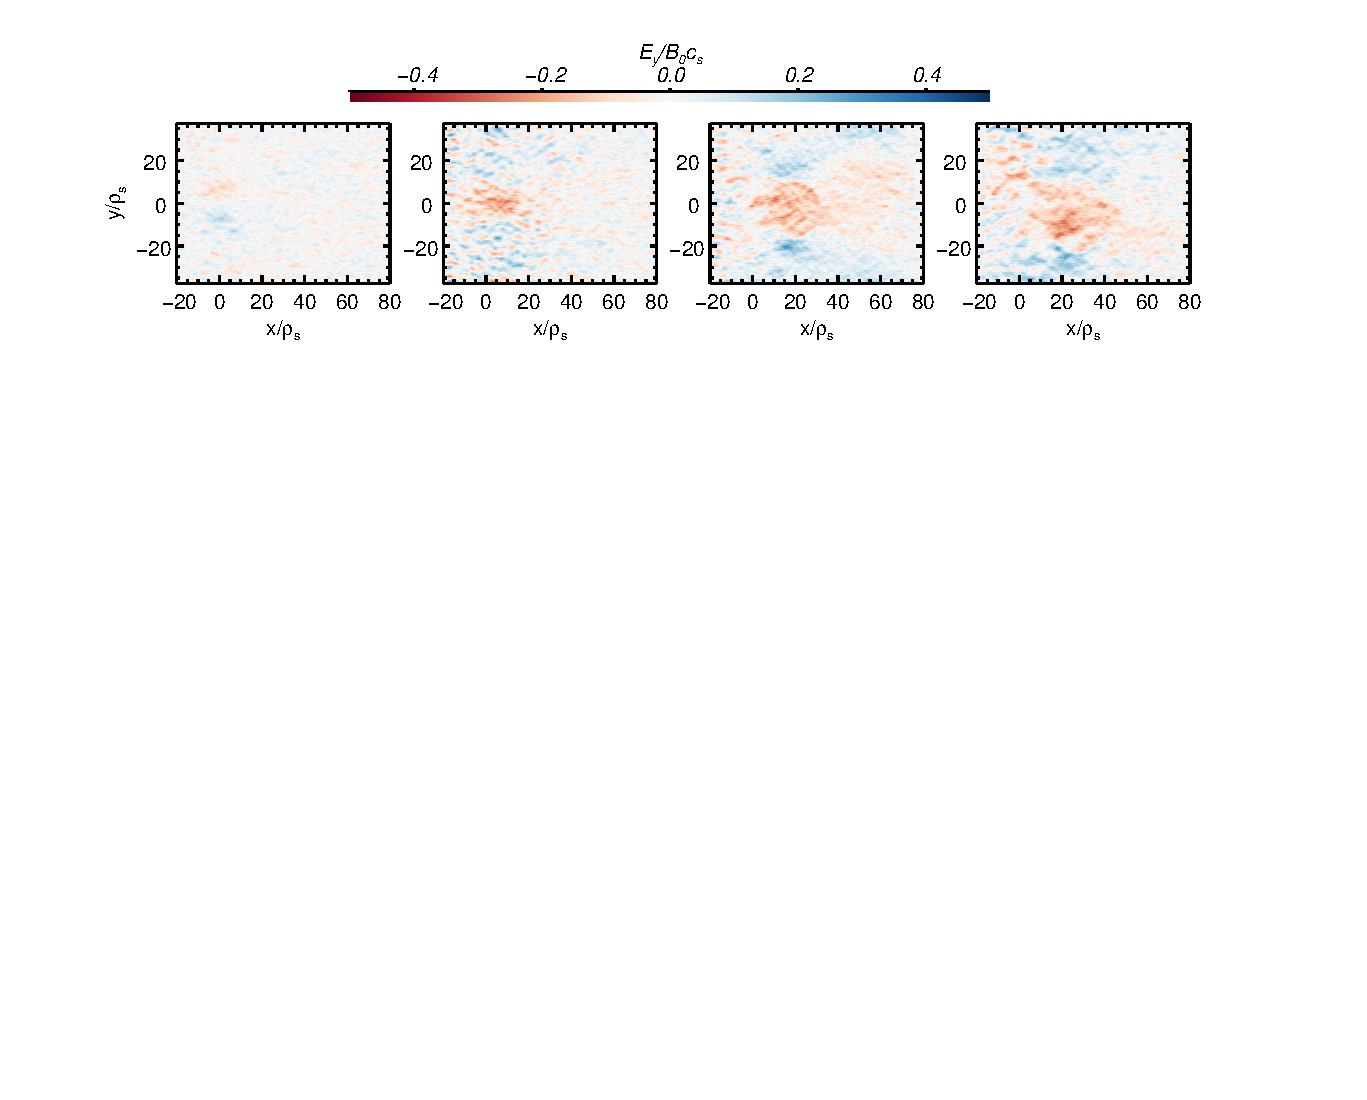
\includegraphics[trim=0mm 128mm 0mm 0mm,width=\textwidth]{Pictures/eytot.eps}
  \caption{Electric field in y-dir at $t\omega_{ci}={6,150,300,450}$}
  \label{efield}
\end{figure*}


The radial driving mechanism is thought to be an initial dipole creation from the gradient in the magnetic field followed by an radial electrical drift. I.e. an overall effect of individual charged particle motion in the inhomogeneous magnetic field. Looking at fig. \ref{pot} we see the gyro-averaged potential at times $t\omega_{ci}={6,150,300,450}$. Comparing with figure \ref{blob} of the blob it is seen that a dipole has en indeed appeared at the position of the blob. 
This potential yields an electric field as seen in fig \ref{efield} (y-component). It is seen that the field within the blob is pointing downwards which combining with the magnetic field pointing into the plane corresponds well with the outward radial propagation. Furthermore, the strengh of the electric field within the blob corresponds well with the radial velocity of the blob estimated to be $v_\perp \approx 0.1c_s$. 

Furthermore, as the blob moves outwards we see a break in the poloidal symmetry of the blob with a movement in the $\grad \fd B\times \fd B$-direction (-y-direction). Note that this is in the opposite direction of what is seen in fluid simulations while consistent with results seen in [Hasegawa] and [Gingell?]. This symmetry breaking has been described in detail in [jens] and is in large part attributed to finite Larmor radius effects as discussed earlier. 

Before we dive into the scaling dependence we look at the basis for the scaling we saw earlier, namely the quasi-neutrality condition. As mentioned, this is not fulfilled at every point in the domain, se particles are 'free' to move around. Instead we introduced a measure to estimate the level of quasi-neutrality. To test this we find the average and maximum deviation from neutrality in a given $\rho_s^2$ area. The result for the run in fig. [the one with the...] is seen in fig. We see that on average (black dots) the charge seperation is below the threshold condition. For the maximum deviation we see that in general it is below the threshold, but with certain spikes breaking it. This does not seem to impose any changes to the overall blob behaviour. Overall this means that we can expect to meet the condition necessary for obtaining the scaling law presented in section !!INSERT!!
x

\begin{figure}[h]
\center
	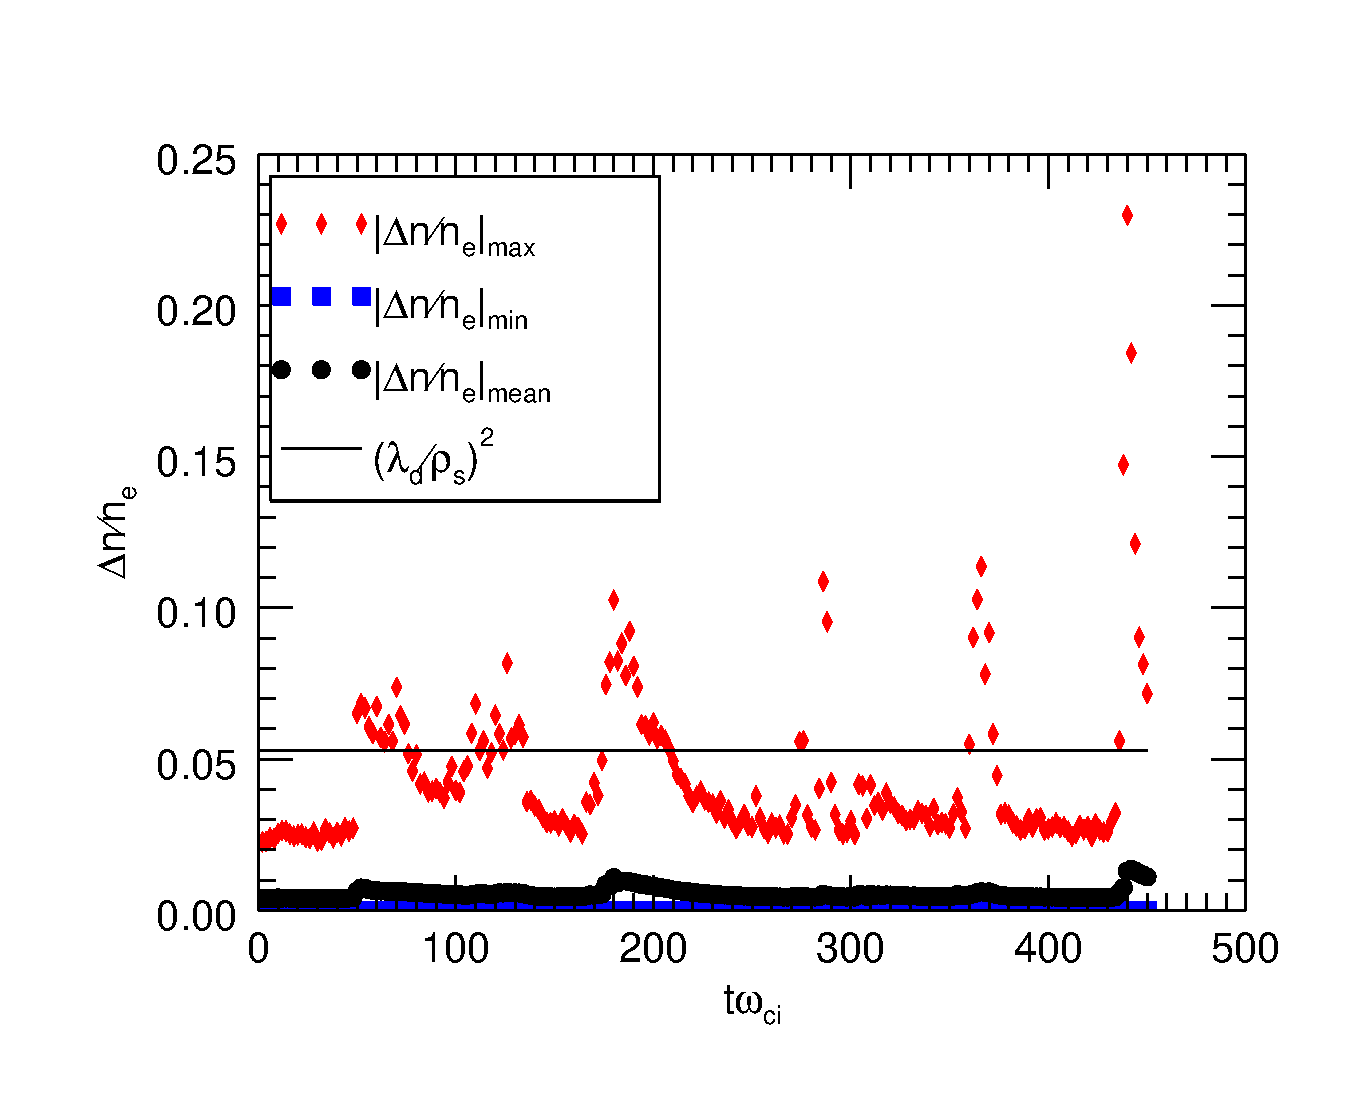
\includegraphics[width=0.5\textwidth]{Pictures/quasineuwl.eps}
\end{figure}

\begin{figure*}
\centering
\begin{subfigure}{.49\textwidth}
	\centering
	\includegraphics[trim={115mm 88mm 1mm 7mm},clip,width=1\linewidth]{Pictures/posxgrpewiitgt.eps}
\end{subfigure}
\begin{subfigure}{.49\textwidth}
	\centering
	\includegraphics[trim={115mm 88mm 1mm 7mm},clip,width=1\linewidth]{Pictures/xnormgrpewiitgt.eps}
\end{subfigure}
\begin{subfigure}{.49\textwidth}
	\centering
	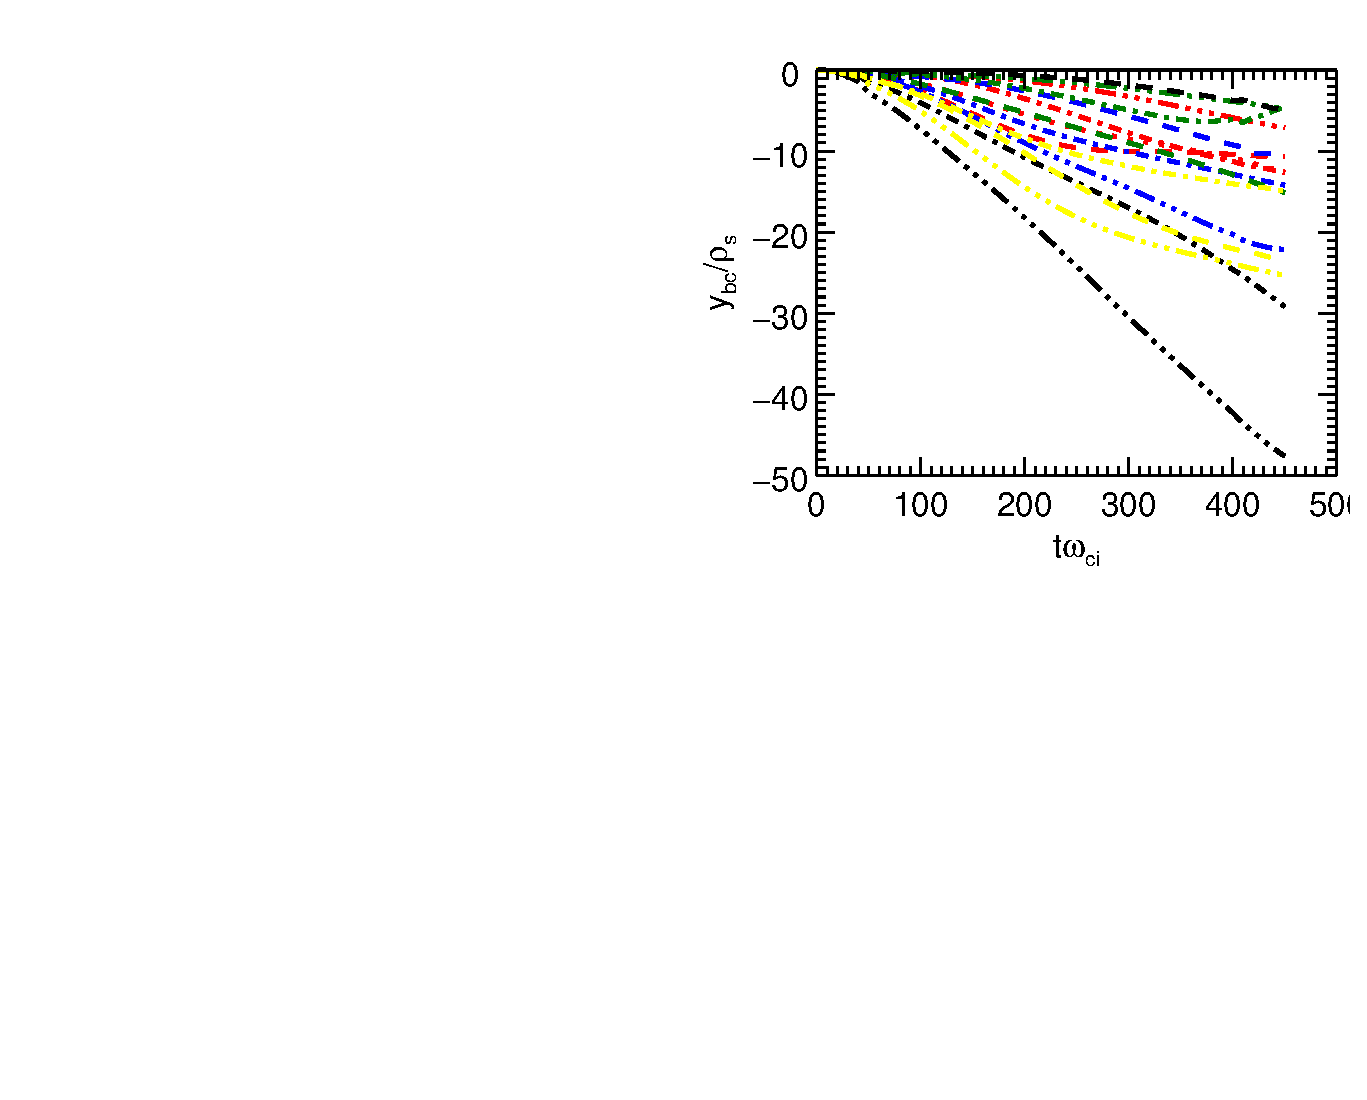
\includegraphics[trim={115mm 88mm 1mm 7mm},clip,width=1\linewidth]{Pictures/posygrpewiitgt.eps}
\end{subfigure}
\begin{subfigure}{.49\textwidth}
	\centering
	\includegraphics[trim={115mm 88mm 1mm 7mm},clip,width=1\linewidth]{Pictures/ynormgrpewiitgt.eps}
\end{subfigure}
\label{scaling}
\end{figure*}


\begin{table}[]
\centering
%\caption{My caption}
\label{my-label}
\begin{adjustbox}{max width=0.7\textwidth}
\begin{tabular}{|l|l|l|l|l|}
\hline
\begin{tabular}[c]{@{}l@{}}Perturb\\ $n_0$\end{tabular} & \begin{tabular}[c]{@{}l@{}}Width\\ $\rho_s$\end{tabular} & \begin{tabular}[c]{@{}l@{}}Temp ratio\\ $T_i/T_e$\end{tabular} & \begin{tabular}[c]{@{}l@{}}Gradient\\ $\rho_s$\end{tabular} & \begin{tabular}[c]{@{}l@{}}Gaussian temp\\ $(i,e)$\end{tabular} \\ \hline
\cellcolor[HTML]{3166FF}{\color[HTML]{FFFFFF} $0.5$}    & \cellcolor[HTML]{32CB00}$2.5$                            & \cellcolor[HTML]{343434}{\color[HTML]{FFFFFF} $0$}             & \cellcolor[HTML]{FD6864}$250$                               & \cellcolor[HTML]{FFFE65}$0,1$                                   \\ \hline
\rowcolor[HTML]{9698ED} 
$1$                                                     & $5$                                                      & $1$                                                            & $500$                                                       & $0,0$                                                           \\ \hline
\cellcolor[HTML]{3166FF}{\color[HTML]{FFFFFF} $2$}      & \cellcolor[HTML]{32CB00}$10$                             & \cellcolor[HTML]{343434}{\color[HTML]{FFFFFF} $3$}             & \cellcolor[HTML]{FD6864}$1000$                              & \cellcolor[HTML]{FFFE65}$1,0$                                   \\ \hline
\cellcolor[HTML]{3166FF}{\color[HTML]{FFFFFF} $4$}      & \cellcolor[HTML]{32CB00}$20$                             & \cellcolor[HTML]{343434}{\color[HTML]{FFFFFF} $7$}             & \cellcolor[HTML]{FD6864}$2000$                              & \cellcolor[HTML]{FFFE65}$1,1$                                   \\ \hline
\end{tabular}
\end{adjustbox}
\label{runs}
\end{table}

\subsection{Scaling}

In figure \ref{scaling} we see the radial and poloidal evolution of the different blobs parameters. The color coding and line style follows table \ref{runs}. An initial observation is that all runs show a radial propagation as well as a poloidal. 

As for the poloidal movement we see that for all runs the blob goes in the $\grad B\times \fd B$-direction indicating that it is a consistent result that can be expected for all runs irrespective of parameters. It is further noted that there seems to be a tedency for the movement to coincide with the size of the blob compared to the larmor radius. E.g. for the ion temperature case that low larmor radius due to $T_i/T_e=0$ (black dash), it is evident that almost no movement in the y-direction is present. On the other hand, higher temperature, $\tau={3,7}$ (black dot dash, 3xdot dash) have much higher movement. This corresponds well with the increasing larmor radius due to temperature dependence [THESE ARE SEEM IN THE RIGHT PICTURES]. Likewise we see the same in the case of varying blob width (green) with larger blob width showing lower y-dir propagation and the more narrow shower larger propagation.

In terms of FLR, what acctually matters?
Looking at the FLR measure we introduced earlier, see fig MAKE AND INSERT, we see that for the perturbation and gradient scalings, the curves follows roughly the same trend while for the width, temperature ratio and to a smaller extend the gausssian temperature perturbation we see clear dependecies. The overall trend points to poloidal propagation being dependent on larmor radius compared to the blob width.  

From fig \ref{scaling} right we see no apparent scaling of the poloidal movement 


The scaling was a general expression for movement perpendicular to the magnetic field however, the above together shows that the scaling only has predictive capabilities in the radial direction and not in the poloidal. This is a as could be expected since in the derivation, no FLR are included to account for this propagation. Likewise when explaining the overall blob driving mechanism it is solely based on drift which are either perpendicular (grad-B drift) or along the radial direction (electric drift).  
\section{Discussion}
We see good scaling results - FLR effects in the y-dir - not the same as all fluid papers.

\section{Conclusion}
Awesome new code to show awesome results.


%\end{multicols}
\end{document}


%   \includegraphics[trim={115mm 88mm 1mm 7mm},clip,width=1\linewidth]{../figures/posxgrpewiitgt.eps}
%   %\caption{Left shows the position in the x-direction (top) and y-direction (bottom). Right shows the $\sigma$ normalized position wrt $\gamma$ normalized time.}
%
%
%   \includegraphics[trim={115mm 88mm 1mm 7mm},clip,width=1\linewidth]{../figures/xnormgrpewiitgt.eps}
%   %\caption{Left shows the velocities of the blob in the x-dir (top) and y-dir (bottom). Right shows the FLR effect measure of $y/x$ (top) and $V_y/V_x$ (bottom).}
%
%
%
%%   \includegraphics[trim={115mm 88mm 1mm 7mm},clip,width=1\linewidth]{../figures/ynormgrpewiitgt.eps}
%%   %\caption{Left shows the velocities of the blob in the x-dir (top) and y-dir (bottom). Right shows the %FLR effect measure of $y/x$ (top) and $V_y/V_x$ (bottom).}
%
%
%
%   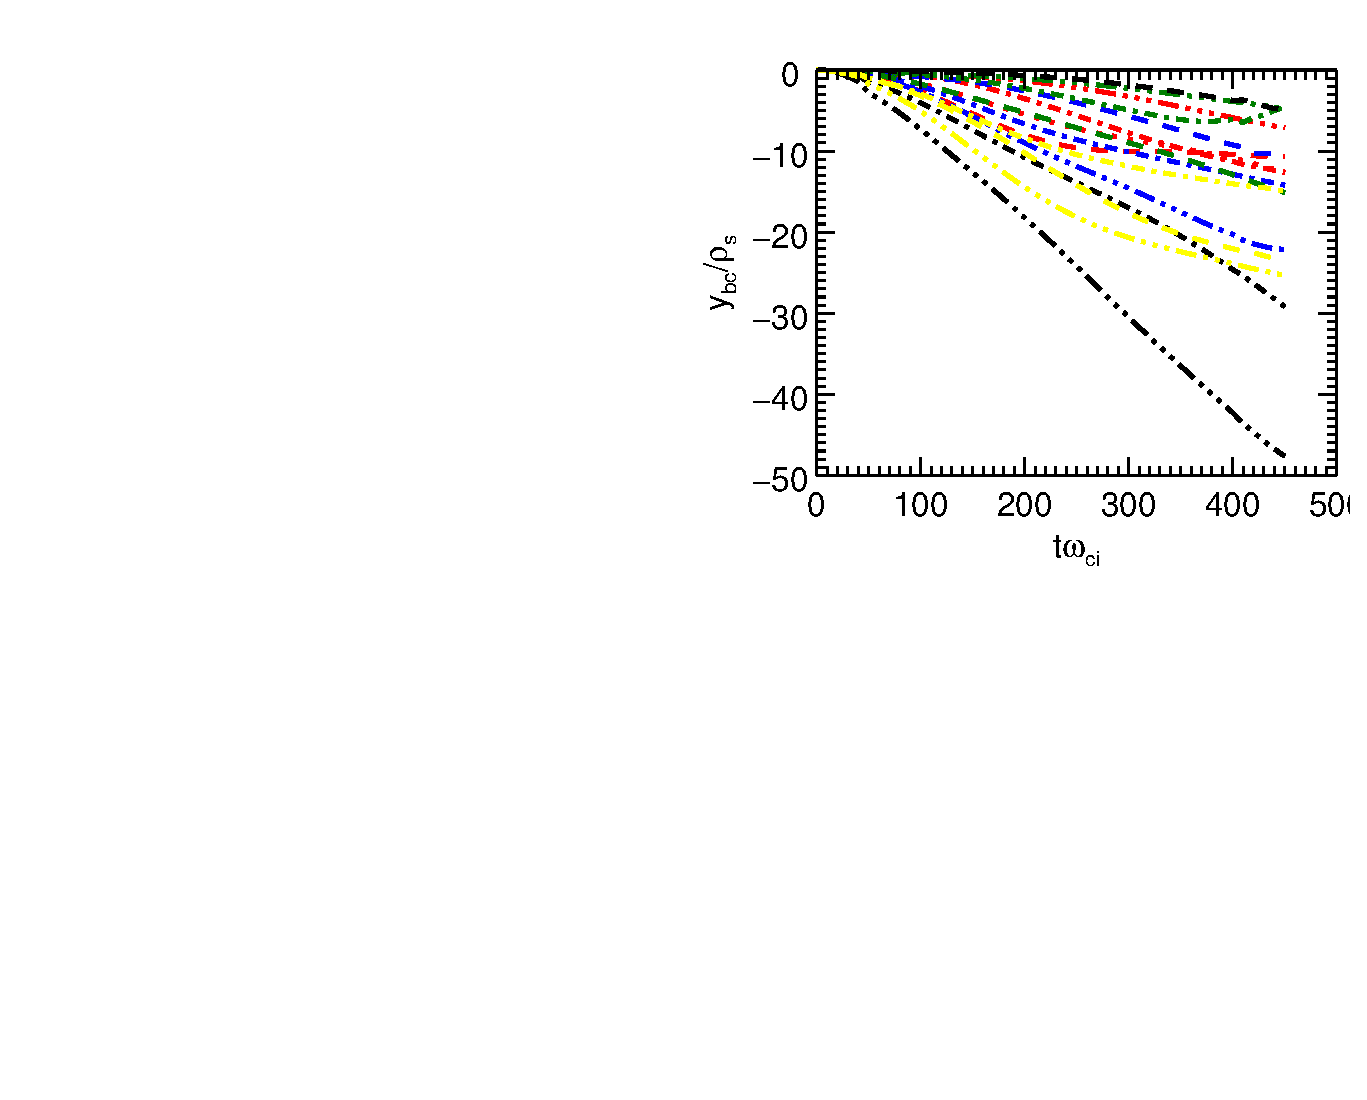
\includegraphics[trim={115mm 88mm 1mm 7mm},clip,width=1\linewidth]{Pictures/posygrpewiitgt.eps}
%   %\caption{Left shows the velocities of the blob in the x-dir (top) and y-dir (bottom). Right shows the FLR effect measure of $y/x$ (top) and $V_y/V_x$ (bottom).}
%   
%
%
%   \includegraphics[trim={115mm 88mm 1mm 7mm},clip,width=1\linewidth]{Pictures/ynormgrpewiitgt.eps}
%   %\caption{Left shows the velocities of the blob in the x-dir (top) and y-dir (bottom). Right shows the FLR effect measure of $y/x$ (top) and $V_y/V_x$ (bottom).}



% ***********************************************************
% ********************** END HEADER *************************
% ***********************************************************